%%%%%%%%%%%%%%%%%%%%%%%%%%%%%%%%%%%%%%%%%%%%%%%%%%%%%%%%%%%%%%%%
%                                                              %
%          GuIT - Gruppo Italiano Utilizzatori di TeX          %
%                                                              %
%          M. Himmelmann, E. Vavassori, F. Busdraghi           %
%                                                              %
%           ---  Introduzione al mondo di LaTeX  ---           %
%                         Versione 1.1                         %
%                                                              %
%     Questo materiale è rilasciato sotto licenza CCPL 2.5     % 
% Consultare la documentazione allegata per maggiori dettagli  %
%                                                              %
%%%%%%%%%%%%%%%%%%%%%%%%%%%%%%%%%%%%%%%%%%%%%%%%%%%%%%%%%%%%%%%%

% vim:sts=2:ts=2:tw=70
\documentclass[svgnames,%
	ucs,% Serve per l'encoding UTF8
	pdftex]{guitbeamer}
\usepackage[utf8x]{inputenc}
\usepackage[greek,italian]{babel}
\languageattribute{greek}{polutoniko}
\graphicspath{{img/}}

% Titolo del corso, autore, data
\title[Introduzione al mondo di \LaTeX]{Introduzione al mondo di \LaTeX}
\author[Maurizio W.\,Himmelmann]{Maurizio W.\,Himmelmann}
\date{30 novembre 2009} % qui ci va anche l'evento

% Si comincia :)
\begin{document}

% Pagina del titolo
\frame{\titlepage}
%-----------------------------------------------------------
%--------------------------------------------------- SLIDE -
\begin{frame}
  \frametitle{Pagina web del corso}
	\begin{center}
	  \large
		\url{http://www.guit.sssup.it/corsi/corso_himmel.php}
	\end{center}
\end{frame}
%-----------------------------------------------------------
%--------------------------------------------------- SLIDE -
\begin{frame}
  \frametitle{Guide gratuite}
	\begin{thebibliography}{Wel66}
		\bibitem [BC07]{BECCARI}
			Beccari, Claudio.
			\newblock \textit{Introduzione all'arte della composizione tipografica}.
			\newblock{\small\url{http://www.guit.sssup.it/downloads/GuidaGuIT.pdf}}
		\bibitem [Pantieri]{Pantieri}
			L.~Pantieri.
			\newblock {\em L'arte di scrivere con {\LaTeX}}, 2009.
			\newblock {\footnotesize\url{http://www.lorenzopantieri.net/LaTeX_files/ArteLaTeX.pdf}}
	\end{thebibliography}
\end{frame}
%-----------------------------------------------------------
%--------------------------------------------------- SLIDE -
\begin{frame}
  \frametitle{Testi avanzati}
	\begin{thebibliography}{Wel66}
		\bibitem [SYR]{SYR}
			Syropoulos, Apostolos; Tsolomitis, Antonis; Sofroniou, Nick.
			\newblock \textit{Digital Typography using \LaTeX}.
		\bibitem [SYR]{SYR}
			Kopka, Helmut; Daly, Patrick W.
			\newblock \textit{A Guide to \LaTeX\ - Document Preparation for
			Beginners and Advanced Users}
	  \bigskip
		\bibitem [KNU]{KNU}
			Knuth, Donald.
			\newblock \textit{The \TeX book}
	\end{thebibliography}
\end{frame}
%-----------------------------------------------------------
%--------------------------------------------------- SLIDE -
% \begin{frame}
%   \frametitle{Articoli specifici}
%   \footnotesize
% 
% \begin{columns}
% \column[t]{.5\textwidth}
% \begin{thebibliography}{Wel66}
%     \bibitem [Mori08b]{Mori08b}
%     L.~F. Mori.
%     \newblock Gestire la bibliografia con {\LaTeX}.
%     \newblock \emph{Ars \TeX nica}, (6), October 2008.
% 
%     \bibitem [Mori08a]{Mori08a}
%     M.~Guiggiani and L.~F. Mori.
%     \newblock Consigli su come \emph{non} maltrattare le formule matematiche.
%     \newblock \emph{Ars \TeX nica}, (5):5--14, April 2008.
% 
%     \bibitem [Mori07a]{Mori07a}
%     L.~F. Mori.
%     \newblock Scrivere la tesi di laurea con {\LaTeXe}.
%     \newblock \emph{Ars \TeX nica}, (3):23--45, April 2007.
% \end{thebibliography}
% \column[t]{.5\textwidth}
% \begin{thebibliography}{Wel66}
%     \bibitem [Mori07b]{Mori07b}
%     L.~F. Mori and M.~W. Himmelmann.
%     \newblock Scrivere il curriculum vitæ con {\LaTeX}.
%     \newblock \emph{Ars \TeX nica}, (4):5--15, October 2007.
% 
%     \bibitem [Mori06]{Mori06}
%     L.~F. Mori.
%     \newblock Tabelle su {\LaTeXe}: pacchetti e metodi da utilizzare.
%     \newblock \emph{Ars \TeX nica}, (2):31--47, October 2006.
% \end{thebibliography}
% \end{columns}
% 
% \end{frame}
%-----------------------------------------------------------
%--------------------------------------------------- SLIDE -
% \begin{frame}
%   \frametitle{Riviste}
% 	\begin{thebibliography}{Wel66}
% \bibitem [Arstexnica]{Arstexnica}
% \Ars
% \newblock \emph{Rivista italiana di \TeX\ e \LaTeX}.
% \newblock \url{http://www.guit.sssup.it/arstexnica/}
% 
% \bibitem [PracTeX]{PracTeX}
% The Prac\TeX\ Journal
% \newblock \emph{The online journal of the \TeX\ Users Group}.
% \newblock \url{http://www.tug.org/pracjourn/}
% 
% \bibitem [TUGboat]{TUGboat}
% TUGboat
% \newblock \emph{The Communications of the \TeX\ Users Group}.
% \newblock \url{http://www.tug.org/TUGboat/}
%     \end{thebibliography}
% \end{frame}
%-----------------------------------------------------------
%--------------------------------------------------- SLIDE -
\begin{frame}
  \frametitle{Piano della presentazione}
  \tableofcontents
\end{frame}
%-----------------------------------------------------------
%--------------------------------------------------- SLIDE -
\begin{frame}
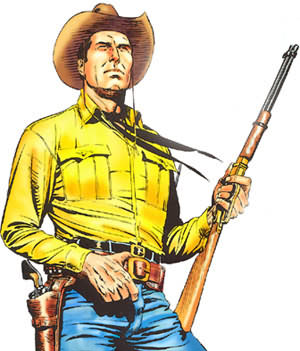
\includegraphics[scale=.5]{texwiller.jpg}

  \itshape
	Mi chiamo Tex Willer e vengo da Palo Verde\dots
	\begin{flushright}
		\upshape
		L. Bonelli, Il mio nome \`e Tex
	\end{flushright}
\end{frame}
%-----------------------------------------------------------
%------------------------------------------------- SECTION -
\section{\TeX\ e \LaTeX}
%-----------------------------------------------------------
%---------------------------------------------- SUBSECTION -
\subsection{La storia di \TeX}
%-----------------------------------------------------------
%--------------------------------------------------- SLIDE -
\begin{frame}
  \frametitle{Perch\'e si chiama \TeX?}
	Il nome deriva dalle prime tre lettere della parola\\[.5cm]
	\begin{center}
		\alert{\large\foreignlanguage{greek}{teqn\'h}}
		(tecnica, arte)\\
		e\\
		\alert{\large\foreignlanguage{greek}{teqnologia}}
		(tecnologia)
	\end{center} 
  \bigskip
	\begin{center}
		L'ultima lettera di \TeX\ e \LaTeX\ deve essere quindi letta
		come il ``\emph{ch}'' di chiave
	\end{center}
\end{frame}
%-----------------------------------------------------------
%--------------------------------------------------- SLIDE -
\begin{frame}
  \frametitle{Ecco chi ha scritto il \TeX}
	\begin{center}
		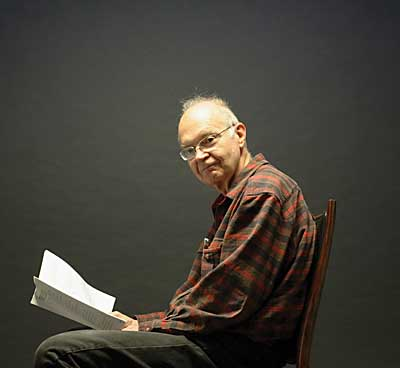
\includegraphics[scale=.5]{knuth}\\[.5em]
		\large Donald E.\ Knuth
	\end{center}
\end{frame}
%-----------------------------------------------------------
%--------------------------------------------------- SLIDE -
\begin{frame}
  \frametitle{Una curiosit\`a\dots}
	Le versioni di \TeX\ non sono identificate con un numero progressivo 
	(es., 2.6.1) bens\`i con il numero di cifre decimali che
	seguono il 3 nella sua approssimazione a $\pi$.
	\begin{center}
		La versione attuale \`e la \textbf{3,141592}
	\end{center}
  \bigskip 
	\begin{block}{Il testamento di Knuth}<2->
	Secondo le sue volont\`a la versione di \TeX\ sar\`a fissata a $\pi$ solo
	al momento della sua scomparsa (e da quel momento non sar\`a pi\`u
	modificato).
	\end{block}
\end{frame}
%-----------------------------------------------------------
%--------------------------------------------------- SLIDE -
\begin{frame}
  \frametitle{Ecco chi ha sviluppato \LaTeX}
	\begin{center}
		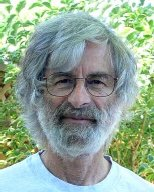
\includegraphics[height=5cm]{leslie}\\[2mm]
		\large Leslie Lamport
	\end{center}
\end{frame}
%-----------------------------------------------------------
%--------------------------------------------------- SLIDE -
\begin{frame}
  \frametitle{\TeX\ \`e il ``motore'' di \LaTeX}
	\begin{center}
		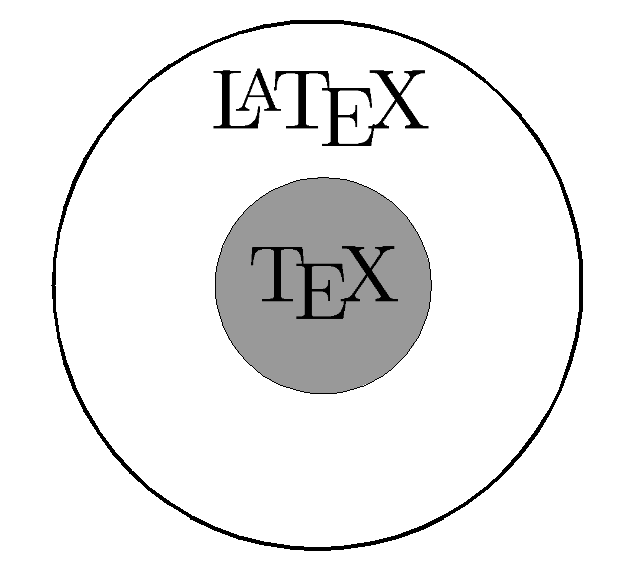
\includegraphics[scale=.4]{texlatex}%
	\end{center}
\end{frame}
%-----------------------------------------------------------
%--------------------------------------------------- SLIDE -
\begin{frame}
  \frametitle{Esistono diverse varianti di \LaTeX}
	\begin{itemize}
		\item\alert{\TeX Live}: multipiattaforma, \`e anche in grado di
			funzionare senza essere installato
		\item\alert{te\TeX} per Unix e GNU/Linux
		\item\alert{MiK\TeX} per Windows
		\item\alert{gw\TeX} per Mac OS X
		\item\alert{Oz\TeX}, \alert{Amiga\TeX}, \dots
	\end{itemize}
  \bigskip
	Tutte queste versioni differiscono tra loro solo per il sistema
	operativo su cui devono essere installate
\end{frame}

%-----------------------------------------------------------
%--------------------------------------------------- SLIDE -
\begin{frame}
  \frametitle{Cosa non \`e \LaTeX}
	\begin{center}
	\LaTeX\ \emph{non \`e} un programma WYSIWYG\\% dire che LaTeX è un programma WYWISYG
	(\textit{what you see is what you get})
	\end{center}
  \bigskip
	A differenza di questo tipo di programmi \textbf{\LaTeX\ non
	possiede un'interfaccia grafica} capace di visualizzare in
	\emph{tempo reale} il documento pronto per la stampa\\
  \bigskip
  \onslide<2->
	\begin{block}{Il concetto di compilazione} 
		La compilazione \`e l'elaborazione di una serie di istruzioni, raccolte in un file di   \emph{input} (puro testo), che produce un file di \emph{output} (per esempio un PDF).
	\end{block}
\end{frame}
%-----------------------------------------------------------
%--------------------------------------------------- SLIDE -
% \begin{frame}
%  \frametitle{Cos'\`e \LaTeX}
% 	\LaTeX\ \`e simultaneamente \textbf{un programma ed un linguaggio} per la composizione tipografica, specificamente concepito per la realizzazione di documenti di elevata qualit\`a finale.\\
%   \bigskip
% 	Contrariamente a quanto si pensa la preparazione di un documento in grado di rispettare precisi canoni estetici \`e un lavoro assai delicato.
% \end{frame}
%-----------------------------------------------------------
%---------------------------------------------- SUBSECTION -
\subsection{La compilazione di un documento}
%-----------------------------------------------------------
%--------------------------------------------------- SLIDE -
% \begin{frame}
%   \frametitle{Il concetto di compilazione} 
% 	La compilazione \`e l'elaborazione di una serie di istruzioni, raccolte in un file di   \emph{input} (puro testo), che produce un file di \emph{output} (per esempio un PDF).\\
%   \bigskip 
% 	Nei programmi WYSIWYG questo avviene in tempo reale. Con \LaTeX\ invece questi due step sono tenuti separati.
%   \medskip
%   \onslide<2->
% 	\begin{block}{Attenzione!}
% 		D'ora in avanti ci riferiremo al file di input chiamandolo con il
% 		termine convenzionale di: \alert{sorgente} 
% 	\end{block}
% \end{frame}
%-----------------------------------------------------------
%--------------------------------------------------- SLIDE -
\begin{frame}
  \frametitle{Il file sorgente}
	Si definisce \textbf{sorgente} del documento il testo del nostro documento
	con all'interno tutte le istruzioni necessarie a \LaTeX\ per
	formattarlo.
  \smallskip
	\begin{center}
		Questo file avr\`a estensione \LCmd[]{.tex}
	\end{center}
  \medskip
  \onslide<2->
	\begin{LaTeXcode}
		Il mio cane Ricky ingoia il registratore e corre tutto il giorno con l'ouverture di \alert{\\textit\{}Guglielmo Tell\alert{\}} in pancia\alert{\\dots}
	\end{LaTeXcode}
  \onslide<3->
	\begin{LaTeXoutput}
		Il mio cane Ricky ingoia il registratore e corre tutto il giorno con l'ouverture di \textit{Guglielmo Tell} in pancia\dots
	\end{LaTeXoutput}
\end{frame}
%-----------------------------------------------------------
%--------------------------------------------------- SLIDE -
\begin{frame}
  \frametitle{Gli \textit{step} di compilazione}
	\begin{center}% I commenti qui sono importanti!
		\includegraphics<1>[height=.8\textheight]{compilazione_1}%
		\includegraphics<2>[height=.8\textheight]{compilazione_2}%
		\includegraphics<3>[height=.8\textheight]{compilazione_3}%
		\includegraphics<4>[height=.8\textheight]{compilazione_4}%
		\includegraphics<5>[height=.8\textheight]{compilazione_5}%
		\includegraphics<6>[height=.8\textheight]{compilazione_6}%
	\end{center}
\end{frame}
%-----------------------------------------------------------
%--------------------------------------------------- SLIDE -
\begin{frame}
  \frametitle{Cosa occorre}
	Ovviamente un compilatore \LaTeX\ (\alert{Mik\TeX}, \alert{te\TeX}, ecc.)\\
  \medskip
  \onslide<2->
	Per scrivere il file sorgente (\LCmd[]{.tex}) \`e consigliabile
	utilizzare un \emph{editor}\/ di testo che aiuti a gestirne la
	compilazione (\alert{Led}, \alert{\TeX nicCenter}, \alert{WinEdt}, \alert{Kile},
	\alert{Emacs}, \alert{\TeX maker}, \alert{Vim\LaTeX suite}, ecc.)\\
  \medskip
  \onslide<3->
	Fanno anche comodo:
	\begin{itemize}
		\item visualizzatore PDF (\alert{Acrobat Reader}, \alert{xpdf}, ecc.)
		\item compilatore PostScript (tipicamente \alert{GhostScript})
		\item visualizzatore PS (\alert{gv}, \alert{KGhostView}, ecc.)	
		\item gestore della bibliografia (\alert{bibtool}, \alert{BibTeXmgr}, ecc.)
		\item \dots
	\end{itemize}
\end{frame}
%-----------------------------------------------------------
%--------------------------------------------------- SLIDE -

\begin{frame}
  \frametitle{Ricapitolando} 
	\begin{itemize}[<+->]
		\item si scrive il sorgente del documento (\LCmd[]{.tex})
		\item si \emph{compila} il sorgente, ovvero dice a \LaTeX\ di trasformare il sorgente in un documento di output (nel nostro caso un \LCmd[]{.pdf})
		\item si legge il documento prodotto con un visualizzatore per \LCmd[]{.pdf}
		\item se si vuole modificare il documento bisogna modificare il	sorgente e ricompilare
	\end{itemize}
\end{frame}
%-----------------------------------------------------------
%--------------------------------------------------- SLIDE -
% \begin{frame}
%   \frametitle{Compito per casa}
%   	\begin{itemize}
% 	\item Scaricare
% 		\begin{itemize}
% 		\item alcune delle guide suggerite
% 		\item i sorgenti degli esempi svolti in classe
% 		\end{itemize}
%   \bigskip
% 	\item Installare
% 		\begin{itemize}
% 		\item una distribuzione (ad es.: MiK\TeX)
% 		\item un editor (ad es.: \TeX nicCenter)
% 		\item la coppia di programmi Ghostscript, GSview
% 		\end{itemize}
%   \bigskip
%   	\item Ripetere gli esercizi fatti in classe
% 	\end{itemize}
% \end{frame}
%-----------------------------------------------------------
%--------------------------------------------------- SLIDE -
\begin{frame}
  \frametitle{Un esempio vale pi\`u di mille parole}
	\begin{center}
		Diamo uno sguardo ai programmi che utilizzeremo
	\end{center}
\end{frame}
%-----------------------------------------------------------
%------------------------------------------------- SECTION -
\section{Cominciamo a lavorare}
%-----------------------------------------------------------
%---------------------------------------------  SUBSECTION -
\subsection{La sintassi dei comandi}
%-----------------------------------------------------------
%--------------------------------------------------- SLIDE -
\begin{frame}
  \frametitle{A che punto siamo}
  \tableofcontents[currentsection,currentsubsection]
\end{frame}
%-----------------------------------------------------------
%--------------------------------------------------- SLIDE -
\begin{frame}
  \frametitle{La sintassi di base}
	\begin{itemize}[<+->]
	\item tutti i comandi cominciano sempre con un
		\LCmd\
	\item spesso il comando \`e il nome inglese dell'azione
	\item il comando ``termina'' con uno spazio bianco o con un
		altro comando:
	\begin{LaTeXcode}<4->
		\\comando \alert{<testo>}\n
		\\comando\\altrocomando
	\end{LaTeXcode}
	\end{itemize}
  \smallskip
	\begin{block}{Attenzione!}<5->
		\LaTeX\ \`e \textit{case sensitive}! Bisogna pertanto stare attenti a distinguere tra\\[.2em]
		\begin{center}
			\alert{\large MAIUSCOLO} e \alert{\large minuscolo}
		\end{center}
	\end{block}
\end{frame}
%-----------------------------------------------------------
%--------------------------------------------------- SLIDE -
\begin{frame}
  \frametitle{I principali tipi di comandi}\small
	Comandi semplici
	\begin{LaTeXcode}<2->
		\\newpage
	\end{LaTeXcode}
  \medskip
	Comandi che richiedono un argomento
	\begin{LaTeXcode}<3->
		\\textit\{\alert{Guglielmo Tell}\}
	\end{LaTeXcode}
  \medskip
  Comandi che richiedono uno (o pi\`u) parametri
	\begin{LaTeXcode}<4->
		\\vspace\{\alert{2cm}\}
	\end{LaTeXcode}
  \bigskip
  \onslide<5->
	Alcuni comandi richiedono di specificare una o pi\`u opzioni:
	\begin{LaTeXcode}
		\\documentclass[\alert{12pt}]\{article\}
	\end{LaTeXcode}
\end{frame}
%-----------------------------------------------------------
%--------------------------------------------------- SLIDE -
\begin{frame}
  \frametitle{Caratteri riservati}
	Esistono poi alcuni caratteri riservati:
	\begin{LaTeXcode}
		\$ \quad \& \quad \% \quad \# \quad \^ \quad \_ \quad \{ \quad \} \quad \~\null
	\end{LaTeXcode}
  \bigskip
	che hanno un significato speciale per \LaTeX\ e che non
	possono essere usati normalmente. Per poterli inserire nel 
	documento dovranno essere tutti preceduti da un \LCmd{} 
\end{frame}
%-----------------------------------------------------------
%--------------------------------------------------- SLIDE -
\begin{frame}
	\frametitle{E il \textit{backslash}?}
	Il \textit{backslash} \`e anch'esso un carattere riservato e per
	scriverlo nel testo si usa il comando:	
	\begin{LaTeXcode}
		\\textbackslash
	\end{LaTeXcode}
\end{frame}
%-----------------------------------------------------------
%--------------------------------------------------- SLIDE -
\begin{frame}
  \frametitle{Scrivere i loghi}
	Ecco come si scrivono i loghi:
	\begin{LaTeXcode}
		\\TeX\n
		\\LaTeX\n
		\\LaTeXe
	\end{LaTeXcode}
  \medskip
	\begin{LaTeXoutput}
		\TeX\\
		\LaTeX\\
		\LaTeXe
	\end{LaTeXoutput}
\end{frame}
%-----------------------------------------------------------
%--------------------------------------------------- SLIDE -
\begin{frame}
  \frametitle{Ambienti}
	Gli \emph{ambienti} sono strutture contraddistinte da
	\begin{LaTeXcode}
		\\begin\{\alert{<nome>}\}\n
		\quad\dots\n
		\\end\{\alert{<nome>}\}
	\end{LaTeXcode}
  \medskip
	Possono essere anche annidati l'uno dentro l'altro a condizione che
	l'ordine di chiusura sia speculare a quello di apertura
\end{frame}
%-----------------------------------------------------------
%---------------------------------------------- SUBSECTION -
\subsection{La struttura dei sorgenti}
%-----------------------------------------------------------
%--------------------------------------------------- SLIDE -
\begin{frame}
  \frametitle{Abbiamo quasi finito}
  \tableofcontents[currentsection,currentsubsection]
\end{frame}
%-----------------------------------------------------------
%--------------------------------------------------- SLIDE -
\begin{frame}
  \frametitle{Il modello di un documento}
	\begin{LaTeXcode}
		\\documentclass\{\alert{<classe>}\}
	\end{LaTeXcode}
\end{frame}
%-----------------------------------------------------------
%--------------------------------------------------- SLIDE -
\begin{frame}
  \frametitle{Le classi base di \LaTeX}
	\begin{LaTeXcode}
		\\documentclass\{\alert{<classe>}\}
	\end{LaTeXcode}
	\begin{itemize}
		\item\Lsty{article}
		\item\Lsty{report}
		\item\Lsty{book}
		\item\Lsty{letter}
		\item\Lsty{slides}
		\item\dots
		\item\Lsty{beamer}
		\item\dots
	\end{itemize}
\end{frame}
%-----------------------------------------------------------
%--------------------------------------------------- SLIDE -
\begin{frame}
  \frametitle{Il modello di un documento}
	\begin{LaTeXcode}
		\\documentclass\{\alert{<classe>}\}\n
	  \onslide<4->
		\hspace*{5ex}\alert{<preambolo>}\nn
	  \onslide<2->
		\\begin\{document\}\n
	  \onslide<3->
		\hspace*{5ex}\alert{<testo del documento>}\n
	  \onslide<2->
		\\end\{document\}
	\end{LaTeXcode}
\end{frame}
%-----------------------------------------------------------
%--------------------------------------------------- SLIDE -
\begin{frame}
  \frametitle{Un esempio vale pi\`u di mille parole}
	\begin{center}
		\alert{\texttt{esempio\_1\_1.tex}}
	\end{center}
\end{frame}
%-----------------------------------------------------------
%--------------------------------------------------- SLIDE -
\begin{frame}
  \frametitle{Le opzioni di \LCmd{documentclass}}
	\begin{LaTeXcode}
		\\documentclass[\alert{<opzioni>}]\{<classe>\}
	\end{LaTeXcode}
	\begin{itemize}
		\item \Lopt{8pt} $\div$ \Lopt{12pt}
		\item \Lopt{a4paper}, \Lopt{a5paper}, \dots
		\item \Lopt{titlepage}%, \Lopt{notitlepage}
		\item \Lopt{twocolumn}%, \Lopt{onecolumn}
		\item \Lopt{twoside}%, \Lopt{oneside}
		\item \dots
	\end{itemize}
  \bigskip
	Le opzioni sono funzionali alla classe di documento prescelta
\end{frame}
%-----------------------------------------------------------
%--------------------------------------------------- SLIDE -
\begin{frame}
  \frametitle{Esempio di classe di documento}
	\begin{LaTeXcode}
		\\documentclass[\alert{a4paper,12pt,twoside}]\{\alert{article}\}
	\end{LaTeXcode}
	Realizza un \emph{articolo} su un foglio \alert{A4} con carattere
	a \alert{12pt} ottimizzato per la stampa \alert{fronte/retro}.
  \bigskip
  \onslide<2->
	\begin{block}{Il bello di \LaTeX}
		Queste impostazioni globali sono modificabili in qualsiasi momento
	\end{block}
\end{frame}
%-----------------------------------------------------------
%--------------------------------------------------- SLIDE -
\begin{frame}
  \frametitle{Commentare il testo}
	Commentare il testo significa renderlo invisibile al processo di
	compilazione, risulta pertanto utile per escludere temporaneamente
	porzioni di testo o codice
	\begin{LaTeXcode}
		\% Prendete una persona, versatele dentro cinque o\n
		sei litri di birra e ne farete un ubriaco
	\end{LaTeXcode}
  \onslide<2->
	\begin{LaTeXoutput}
		sei litri di birra e ne farete un ubriaco
	\end{LaTeXoutput}
  \onslide<3->
	\begin{block}{Attenzione!}
		Il commento \`e valido solo fino alla fine della riga!
	\end{block}
\end{frame}
%-----------------------------------------------------------
%--------------------------------------------------- SLIDE -
\begin{frame}
  \frametitle{I file di stile}
	\LaTeX\ ha una struttura modulare e prevede la possibilit\`a di
	caricare delle \textbf{funzionalit\`a aggiuntive} (\textit{package},
	pacchetti o moduli di estensione) alle funzionalit\`a gi\`a disponibili
	nella dotazione di base ed indispensabili per ottenere determinate
	\emph{feature}.\\
  \bigskip
  \onslide<2->
	I pacchetti hanno estensione \LCmd[]{.sty} e vanno richiamati all'interno del preambolo con il comando:
	\begin{LaTeXcode}
		\\usepackage\{\alert{<nomepkg>}\}\
	\end{LaTeXcode}
  \medskip
  \onslide<3->
	\begin{LaTeXcode}
		\\usepackage[\alert{<opzioni>}]\{<nomepkg>\}\
	\end{LaTeXcode}
\end{frame}
%-----------------------------------------------------------
%--------------------------------------------------- SLIDE -
\begin{frame}
  \frametitle{Due esempi di pacchetti}
	\begin{LaTeXcode}
		\\usepackage\{\alert{graphicx}\}
	\end{LaTeXcode}
	\Lsty{graphicx} \`e un pacchetto che permette di gestire l'inserimento
	delle immagini, dei colori e di rotazioni
  \bigskip
  \onslide<2->
	\begin{LaTeXcode}
		\\usepackage[\alert{italian}]\{\alert{babel}\}
	\end{LaTeXcode}
	\Lsty{babel} permette di sillabare testi scritti in lingue diverse 
	dall'inglese (default), attivando la sillabazione della lingua
	selezionata (in questo caso, la nostra: \LCmd[]{italian})
\end{frame}
%-----------------------------------------------------------
%--------------------------------------------------- SLIDE -
\begin{frame}
  \frametitle{Un esempio vale pi\`u di mille parole}
	\begin{center}
		\alert{\texttt{esempio\_1\_2.tex}}
	\end{center}
\end{frame}
%-----------------------------------------------------------
%--------------------------------------------------- SLIDE -
\begin{frame}
  \frametitle{Utilizzare \textit{packages} aggiuntivi}
	Per potere essere utilizzati i pacchetti devono essere resi
	disponibili al sistema \LaTeX. Per questo esistono due soluzioni:
	\begin{itemize}
		\item copiare il file \LCmd[]{package.sty} nella stessa cartella dove si trova il file \LCmd[]{.tex} da compilare (da evitare)
		\item installare il pacchetto nella distribuzione (fortemente consigliato)
	\end{itemize}
\end{frame}
%-----------------------------------------------------------
%--------------------------------------------------- SLIDE -
\begin{frame}
  \frametitle{Un esempio vale pi\`u di mille parole}
	\begin{center}
		\alert{\texttt{esempio\_1\_3.tex}}
	\end{center}
\end{frame}
%-----------------------------------------------------------
%--------------------------------------------------- SLIDE -
\begin{frame}
  \frametitle{L'encoding di un documento}
	A causa della sua vocazione multipiattaforma e multilingua di \LaTeX, \`e necessario specificare nel sorgente la codifica usata dal vostro computer per definire alcuni caratteri particolari (nel nostro specifico caso le vocali accentate). Questo sistema di codifica prende il nome di \emph{encoding}.\\
  \smallskip
  \onslide<2->
	Quello che utilizziamo nello standard europeo \`e l'\textbf{ISO-8859-15}
  \onslide<3->
	\begin{block}{Attenzione!}
		La codifica da specificare dipende \emph{anche} dal programma utilizzato per scrivere
	\end{block}
\end{frame}
%-----------------------------------------------------------
%--------------------------------------------------- SLIDE -
\begin{frame}
  \frametitle{I principali \textit{encoding} e \LCmd[]{inputenc}}
	\begin{block}{}
	\begin{tabular}{r@{$\quad\Longrightarrow\quad$}l}
		ISO-8859-1 & \onslide<2->{\LCmd[]{latin1}} \\
		ISO-8859-15 & \onslide<2->{\LCmd[]{latin9}} \\
		UTF-8 & \onslide<2->{\LCmd[]{utf8}, \LCmd[]{utf8x}\footnote{richiede
		\Lsty{unicode}}} \\
		Codepage 1252 (Windows) & \onslide<3->{\LCmd[]{ansinew}} \\
		MacRoman (Mac OS X) & \onslide<3->{\LCmd[]{applemac}} \\
	\end{tabular}
	\end{block}
  \onslide<4->
	Per piattaforma Windows
	\begin{LaTeXcode}
		\\usepackage[\alert{latin1}]\{inputenc\}
	\end{LaTeXcode}
  \onslide<5->
	Per piattaform *nix
	\begin{LaTeXcode}
		\\usepackage[\alert{utf8x}]\{inputenc\}
	\end{LaTeXcode}
\end{frame}
%-----------------------------------------------------------
%------------------------------------------------- SECTION -
\section{Perch\'e scegliere \LaTeX}
%-----------------------------------------------------------
%--------------------------------------------------- SLIDE -
\begin{frame}
  \frametitle{A che punto siamo}
  \tableofcontents[currentsection,currentsubsection]
\end{frame}
%-----------------------------------------------------------
%--------------------------------------------------- SLIDE -
\begin{frame}
  \frametitle{Miti sfatati: meglio gli editor WYSIWYG}
	La cosa scomoda di \LaTeX\ \`e che non vedi quello che ottieni\dots
  \medskip
	\begin{block}{La verit\`a}
		\begin{itemize}
			\item con \LaTeX\ non ci sono distrazioni, \`e possibile finalmente pensare solo ai contenuti
			\item scrivere in \LaTeX\ aiuta a strutturare meglio il proprio lavoro, rendendolo pi\`u chiaro
			\item se necessario \`e possibile comunque controllare il \textit{layout} come (anzi, meglio) che in Word
		\end{itemize}
	\end{block}
\end{frame}
%-----------------------------------------------------------
%--------------------------------------------------- SLIDE -
\begin{frame}
  \frametitle{Miti sfatati: lo posso fare con Word}
	Anche Word permette di definire una bibliografia dinamica, comandi di sezionamento, etc.
  \medskip
	\begin{block}{La verit\`a}
		\begin{itemize}
			\item cattive abitudini: meno dell'1\% degli utenti scrive una vera sezione invece di ``Sezione 1''
			\item \LaTeX\ offre un controllo pi\`u profondo e vasto, \`e possibile anche scrivere musica o riviste di scacchi
			\item le macro \LaTeX\ funzionano meglio: vogliamo fare una gara sul posizionamento delle figure?
		\end{itemize}
	\end{block}
\end{frame}
% -----------------------------------------------------------
%--------------------------------------------------- SLIDE -
\begin{frame}
  \frametitle{Miti sfatati: \LaTeX\ \`e difficile} 
	Un amico fisico teorico che studia teoria delle super-stringhe mi ha detto che non vuole imparare \LaTeX\ perch\'e \`e difficile\dots
  \medskip
	\begin{block}{La verit\`a}
		\begin{itemize}
			\item Difficile \`e capire perch\'e stampando Word sposta le figure dove gli pare
			\item non ci vuole una grande fantasia per capire cosa fanno i comandi \LCmd{section} o \LCmd{footnote}
			\item se quello che facciamo ogni giorno fosse semplice come \LaTeX\ avremmo tutti il premio Nobel
		\end{itemize}
	\end{block}
  \smallskip
  \onslide<2->
	\begin{block}{}
		Ci\`o che \`e veramente difficile \`e realizzare documenti disomogenei e non strutturati
	\end{block}
\end{frame}

%-----------------------------------------------------------
%--------------------------------------------------- SLIDE -
\begin{frame}
  \frametitle{Per oggi abbiamo finito}
	\begin{center}
	  \huge
		Grazie e alla prossima lezione
	\end{center}
  \medskip
	\begin{block}{Cosa impareremo la prossima volta}
		\begin{itemize}
			\item qualche cenno sulle \textbf{norme tipografiche} 
			\item \textbf{la struttura} di un documento
			\item \textbf{riferimenti incrociati} per trasformare il vostro documento in un ipertesto
			\item \textbf{curriculum vit\ae} per fare un figurone con vostro nuovo datore di lavoro
		\end{itemize}
	\end{block}
\end{frame}
%-----------------------------------------------------------
%----------------------------------------------------- END -
\end{document}




